\section{Experimental Procedure}\label{sec:exp}
The Digital Electronics Lab is meant to be very open in implementation. The aim will be to build an automated cooling system. We will guide you through this process step by step, but you are also encouraged to bring in your own ideas of other possible implementations!
%
% MATERIAL BEGIN ------------------------------------------------
\subsection{Experimental Material}\label{sec:material}
The full setup is contained in the box shown in \ar{fig:box}. You will find this box on your assigned lab space in room H 41 in the HPP building. The box contains the items shown in \ar{fig:items}, and the contents of the Grove starter kit are shown in \ar{fig:grv}. Manuals for several devices may be found in \ar{tab:man}:\par
%
\fig{.6}{setup0}[Utz box containing the full setup.][fig:box][Utz box with full setup]
%
\fig{1}{setup1}[Content of the Utz box.][fig:items]
%
\fig{1}{setup2}[Content of the Grove starter kit. The base shield is under the red protective foam.][fig:grv][Content of the Grove starter kit.]
\nicetab{ccc}{\textbf{Item} & \textbf{Type} & \textbf{Manual} \\\hline
  multimeter      & UT61C & \href{https://www.distrelec.ch/Web/Downloads/nu/al/UT61_eng_manual.pdf}{Link} \\
  4-pin fan       & Noctua NF-A14 5V PWM & \href{https://noctua.at/en/products/fan/nf-a14-5v-pwm/faq}{Link} \\
  \ac{op-amp}     & LM358 & \href{http://www.ti.com/lit/ds/symlink/lm158-n.pdf}{Link} \\
%   NPN transistor  & BC547 & \href{https://www.sparkfun.com/datasheets/Components/BC546.pdf}{Link} \\
  \ac{NTC} thermistor & B57164-K104-J & \href{https://eu.mouser.com/datasheet/2/400/NTC_Leaded_disks_K164-1317145.pdf}{Link}\\
}[Item manuals.][tab:man]
%
\begin{note}[Lab notes]
  In addition you should bring a lab book (or any other form of notepad) to note down everything what you do and measure (immediately after the execution). Please write clearly and meticulously since it will greatly help you to find mistakes and to write your report! 
\end{note}
%
\begin{note}[Tidy return]
  If you finish your experiment, please return the setup as shown in \ar{fig:box}, \ar{fig:items} and \ar{fig:grv}. If anything broke during the experiment, please inform the assistant, so that it can be replaced.
\end{note}
% MATERIAL END --------------------------------------------------
%
% HOME BEGIN ----------------------------------------------------
\subsection{Working from home}
Due to the compactness of the setup it is possible for you to bring the setup to your place and do the measurements at home. In order to do so, please fill the form and send it signed to the assistant. It is, of course, also possible to do the experiment at the designated lab space at ETH.\par
%
The setup should contain all required items for the experiment. If something is missing or you require additional parts, please contact the technical assistants at the help-desk in HPP J 14. If you want to take additional parts home, please also contact the assistant.\par
% HOME END ------------------------------------------------------
%
% ARDUINO BEGIN -------------------------------------------------
\subsection{Setting up the Arduino}\label{sec:setup}
%
We highly recommend you to install the Arduino \ac{IDE} on your machine so that you can access it any time. If you should have trouble with the installation or you prefer not to use your computer for the experiment, you can use one of the Windows XP machines provided to you at the lab place, which have the Arduino IDE and all necessary drivers pre-installed. These machines do not have internet connection, so you have to bring a portable USB drive to copy the data.
%
\begin{task}[IDE installation]
  Install the Arduino \ac{IDE} following \ar{sec:soft}!
\end{task}
%
\begin{task}[Connecting the Arduino]
  Connect the Arduino to your computer via the \ac{USB} cable and check if it is recognised by the \ac{IDE}!
  \begin{itemize}
    \item select the correct port: \fpath{Tools > Port}
    \item get board info: \fpath{Tools > Get Board Info}
  \end{itemize}
\end{task}
% ARDUINO END ---------------------------------------------------
%
% SKETCH BEGIN --------------------------------------------------
\subsection{Your First Sketch}
In order to have a better overview of your own sketches, it is recommended to set up your own sketchbook location: \fpath{File > Preferences > Sketchbook Location}.
%
\begin{task}[Creating the first sketch]
  \item Create a new sketch with \fpath{File > New}!
\end{task}
%
A new sketch will look like this:
\begin{minted}[linenos]{arduino}
void setup() {
  // put your setup code here, to run once:

}

void loop() {
  // put your main code here, to run repeatedly:

}
\end{minted}
%
Now we want to turn on the LED on the Arduino board, which is connected to the special pin \mintinline{arduino}{LED_BUILTIN}. Since this pin is used as an output, we have to set the \mintinline{arduino}{pinMode} during the \mintinline{arduino}{setup()} function to \mintinline{arduino}{OUTPUT}. Afterwards we can use the \mintinline{arduino}{digitalWrite()} method to set the pin to \mintinline{arduino}{HIGH} (corresponding to \SI{5}{\V}), which will turn on the LED on the board. There is no need to use the \mintinline{arduino}{loop()} function for this simple sketch, but it will be important later.
%
\begin{minted}[linenos]{arduino}
void setup() {
  pinMode(LED_BUILTIN, OUTPUT);
  digitalWrite(LED_BUILTIN, HIGH);
}

void loop() {
  // put your main code here, to run repeatedly:

}
\end{minted}
%
That's it. All the methods and constants used in this script are already defined and do not have to be imported explicitly. There is a long list of such predefined constants. Make sure to not redefine them when adding new constants or variables!
We are now ready to test the communication of the Arduino board with the computer and test if flashing the code works. Make sure to select the correct port and choose \fpath{Arduino/Genuino Uno} as board type if it is not already selected.\newline
%
\begin{task}[Uploading the first sketch]
  First compile the code and then upload it to the Arduino. If everything is working, create a git repository in your sketch folder and commit your first sketch!
\end{task}
%
\begin{note}[Do not use pins A4 \& A5]
  The Arduino Uno uses pins A4 and A5 for the \ac{I2C} communication, which will later be used for the display! Even if it looks like they are separate pins on the shield board, they are shared internally!
\end{note}
% SKETCH END ----------------------------------------------------
%
% BLINK BEGIN ---------------------------------------------------
\subsection{Blinking LED on Bread Board}\label{sec:led}
That was easy (but boring \ldots). As the next step we want to have a blinking external LED on the breadboard. Since it should continue blinking forever, we will use the \mintinline{arduino}{loop()} function now.
%

\begin{task}[Writing a blinking LED sketch]
  Fist supply the breadboard with a voltage of \SI{5}{\V} from the Arduino. Then connect a LED to the breadboard with an appropriate series resistor (\SI{220}{\ohm}) and to a digital pin of the Arduino. Finally write a sketch (\path{Blink.ino}), that makes the LED blink with a frequency of \SI{1}{\Hz} using the \mintinline{arduino}{delay(int nMilliSeconds)} method, which pauses the execution for \mintinline{arduino}{nMilliSeconds}. Upload your sketch now to the Arduino and test it!
\end{task}
%
\begin{task}[Adding a second LED]\label{tsk:bla}
  Now connect a second LED on the breadboard to a different pin. Write a sketch (\path{Blink2.ino}) that makes the second LED blink in a different pattern than the first one, upload it and test it.
\end{task}
%
Why is \mintinline{arduino}{delay()} not the optimal method for this task? Try to use a timer with \mintinline{arduino}{micros()}, which returns a micro-seconds counter as \mintinline{arduino}{unsigned long} to solve this problem. In order to save the result from \mintinline{arduino}{micros} you have to save it to a \mintinline{arduino}{unsiged long} variable. After \SI{\sim 70}{\minute}, the 32-bit counter will overflow and start again from 0! Make sure to handle this case well!
%
\begin{task}[Adding code to the report]
  If you succeeded to implement the two blinking LEDs with timers, please add the code to your report and to your git repository.
\end{task}
% BLINK END -----------------------------------------------------
%
% TIPS BEGIN ----------------------------------------------------
\subsection{General tips for writing code for the Arduino}\label{sec:codestyle}
%
\subsubsection{Data types}
Data types on Arduino are defined differently than for 32-bit or 64-bit x86 processors, e.g. \mintinline{arduino}{int} is only 16-bit, which can store values from -32768 to 32767. In most cases it is better to use \mintinline{arduino}{long} instead of \mintinline{arduino}{int} to avoid overflows. If no negative numbers are required, use \mintinline{arduino}{unsigned} versions. Note: On Arduino Uno, \mintinline{arduino}{double} and \mintinline{arduino}{float} are exactly the same.

\nicetab{lll}{
  \textbf{Type}                       & \textbf{Size} & \textbf{Range}            \\\hline
  \mintinline{arduino}{char}          & 8-bit         & \SIrange{-128}{127}{}     \\
  \mintinline{arduino}{unsigned char} & 8-bit         & \SIrange{0}{255}{}        \\
  \mintinline{arduino}{int}           & 16-bit        & \SIrange{-32768}{32767}{} \\
  \mintinline{arduino}{unsigned int}  & 16-bit        & \SIrange{0}{65535}{}      \\
  \mintinline{arduino}{long}          & 32-bit        & \SIrange{-2147483648}{2147483647}{}  \\
  \mintinline{arduino}{unsigned long} & 32-bit        & \SIrange{0}{4294967295}{} \\
  \mintinline{arduino}{float}         & 32-bit        & floating point            \\
  \mintinline{arduino}{double}        & 32-bit        & floating point            \\
}[Basic numeric data types for the Arduino Uno.][tab:1]
%
\begin{note}[Datatypes]
  Be sure to use \mintinline{arduino}{unsigned long} to store the output of microsecond counters like \mintinline{arduino}{micros()}!
\end{note}
%
\subsubsection{Avoid hard-coded values}
Avoid of a ``hard-coded'' numbers somewhere in the middle of your program, like \eg
%
\begin{minted}[linenos]{arduino}
...
if (now > lastPid + 100000) {
...
\end{minted}
%
Rather define a constant (with \mintinline{arduino}{const} or as a macro with \mintinline{arduino}{#define} in the beginning of the program. Give it a systematic name, like all uppercase for constants, include the unit (\eg micro-seconds) and add a comment: 
%
\begin{minted}[linenos]{arduino}
#define INTERVAL_MICROS_PID 100000 // update interval of PID in micro-seconds
...
if (now > lastPid + INTERVAL_MICROS_PID) {
...
\end{minted}
%
and then use the constant (\mintinline{arduino}{INTERVAL_MICROS_PID}) in the \mintinline{arduino}{if} clause. This makes the code easier to read. Macros with \mintinline{arduino}{#define} do not use space for variables (in contrast to a declaration with \mintinline{arduino}{int ...}), which reduces the memory footprint of your program. Keep in mind that the total RAM is only \SI{2}{\kilo\byte}, which corresponds to only around 500 32-bit integers that you can store! Note, that part of this memory is already used by libraries. Using constants instead of hard-coded numbers is especially important for pin numbers.\par
%
\subsubsection{Code documentation}
Add a short description on the functionality of your program at the top of the code. Include the date and author name. Also comment any non-trivial steps in your code. (Remember: it is in general better to write code in a self-explaining way, such that no comments are necessary. Sometimes though, comments are unavoidable.) \newline
%
\begin{task}[Code documentation]
  Always add reasonable documentation to your code, so that it is easy for another person to understand each step of it!
\end{task}
% TIPS END ------------------------------------------------------
%
% T-GROVE BEGIN -------------------------------------------------
\subsection{Grove Temperature Sensor}\label{sec:grovetemp}
In this experiment you will work with the \href{http://wiki.seeedstudio.com/Grove-Temperature_Sensor_V1.2/}{Grove - Temperature Sensor V1.2}. It uses a \ac{NTC} thermistor to detect the ambient temperature. The specifications of the sensor are shown in \ar{tab:gt}.
%
\nicetab{ll}{
  \textbf{Specification}      & \textbf{Value}                \\\hline
  Operating voltage           & \SIrange{3.3}{5.0}{\volt}     \\
  Zero power resistance       & \SI{100\pm1}{\kilo\ohm}       \\
  Operating temperature range & \SIrange{-40}{+125}{\celsius} \\
  Nominal $B$-constant        & \SIrange{4250}{4299}{K}       \\
}[Specifications of the Grove-Temperature Sensor V1.2.][tab:gt]
%
\begin{task}[Connecting the Grove temperature sensor]
  First connect the Grove Base Shield to your Arduino. Then find out which connector on the shied you have to use to connect the temperature sensor.
\end{task}
%
\begin{task}[Measuring the ambient temperature]
  Create a new sketch and name it \path{GroveTemp.ino}! In order to measure the temperature, you have to first read the voltage value from the sensor, then convert the voltage into the corresponding resistance and then convert the resistance to a temperature in \si{\celsius}. Use the serial interface to write one temperature reading every second and both investigate the data with the \textit{Arduino Serial Monitor}: \fpath{Tools > Serial Monitor} (\code{Ctrl+Shift+M}) and the \textit{Arduino Serial Plotter}: \fpath{Tools > Serial Plotter} (\code{Ctrl+Shift+P})
\end{task}
%
\begin{note}[Baud rate]
  The serial connection has to be enabled during the \mintinline{arduino}{setup()} function with \mintinline{arduino}{Serial.begin(9600);} where 9600 is the baud rate. 9600 is the default value for the \textit{Arduino Serial Plotter} and \textit{Arduino Serial Monitor} utilities, so it is convenient to use this.
\end{note}
% T-GROVE END ---------------------------------------------------
%
% GROVE-3 BEGIN -------------------------------------------------
\subsection{Grove Display and Potentiometer}\label{sec:grovedisp}
As a next step, we will add two more components from the Grove kit: an LCD display to show the current temperature reading of the sensor and a potentiometer to adjust the threshold for our two-point temperature control later. 
%
\begin{task}[Adding a LCD display]
  First install the libraries from the \href{http://wiki.seeedstudio.com/Grove-LCD_RGB_Backlight/}{Grove website}. Include the libraries to your sketch and initialise the display in the \mintinline{arduino}{setup()} function, based on the example code on the above website. Connect the Grove LCD RGB Backlight display to your Grove Shield and modify your project, such that the measured temperature is printed on the display and updated every second.
\end{task}
%
\begin{note}[VCC switch]
  The LCD display will only work correctly, if the \textit{3V3\_VCC\_5V} switch on the Grove Shield is setup to \SI{5}{\V}.
\end{note}
%
\begin{task}[Temperature threshold]
  \begin{enumerate}
    \item Define a fixed threshold in your code, \eg \SI{30}{\celsius}, above which a LED is turned on. As an alternative you can also change the background colour of the display. (Always test if your code is working!)
    \item Make the threshold adjustable without recompiling the code! For this purpose, connect a potentiometer, \eg the Grove Rotary Angle Sensor, to the Grove Shield. Using the \href{http://wiki.seeedstudio.com/Grove-Rotary_Angle_Sensor/}{description}, read out the sensor with \mintinline{arduino}{analogRead()} and map the \ac{ADC} values (\SIrange{0}{1023}{}) to a reasonable temperature range (a$\,\sim\, $b), \eg \SIrange{20}{40}{\celsius}. This can be  implemented, \eg, with the method  \mintinline{arduino}{map(adc, 0, 1023, a, b)}.
    \item Indicate the status (below/above threshold) also in the output to the serial interface. For example, add a second number (0 = below threshold, 50 = above threshold) separated by a space.
    \item Test your code by setting the threshold below and above the room temperature! The serial plotter should now draw a second line indicating whether the value is below or above threshold. Vary the threshold slowly below and above the room temperature and make a screenshot of the resulting graph.
    \item (Optional). Print the temperature threshold on the second row of the display below the measured temperature!
    \item Add the code to your report!
  \end{enumerate}
\end{task}
% GROVE-3 END ---------------------------------------------------
%
% DATA BEGIN ----------------------------------------------------
\subsection{Data handling}\label{sec:data}
Even though the Arduino \ac{IDE} has tools to display the values from the temperature sensor, there is no way to save them. That is why we encourage you to write a short program to save the data to file, so that you can analyse it afterwards. We recommend you to use python for this purpose, but feel free to use whatever you have the most experience with.\par
%
Once a sketch is uploaded to the microprocessor, the Arduino will perform the loop until it is disconnected from power or overwritten by a new sketch. Note down the port number or name, which can be seen under \fpath{Tools} in the Arduino \ac{IDE}. In order to read the data externally from the serial port you have to close the Arduino serial tools (Serial Monitor, Serial Plotter, \ldots).\par
%
\subsubsection{Python}
Python needs the \mintinline[style=default]{python}{pyserial} package to be able to read from the serial interface.\par
%
\noindent If you are using \textbf{anaconda}, type the following command in your anaconda shell:
%
\begin{minted}{console}
student@host:~$ conda install -c anaconda pyserial
\end{minted}
%
\noindent If you are using \textbf{pip}:
\begin{minted}{console}
student@host:~$ sudo pip install pyserial
\end{minted}
%
You can test if you have installed the \mintinline[style=default]{python}{pyserial} package correctly by typing \mintinline[style=default]{python}{import serial} into a python shell. If this works, you can start writing you python code. An outline of what the code should do is below (python3):
%
\mdfsetblack
\begin{minted}{python}
  #!/usr/bin/python3
  
  from serial import Serial
  
  port_name = '<arduino_portname>'  # the name of the port is shown in the IDE
  arduino = Serial(portname)  # open serial port of the Arduino
  
  line = arduino.readline()  # read a single line of the serial output
  
  def save_line(file_name):  
    """ writes a single temperature measurement to the next line of the file [file_name] ."""
    pass
    
  def save_data(file_name):
    """ opens a file [file_name] and continues to save the data. """
    pass
    
  def add_timestamp(line):  # optional
    """ adds the current time stamp to the [line] to simplify the analysis. """
    from datetime import datetime
    t = str(datetime.now())
\end{minted}
%
If you have trouble handling files in python follow this \href{http://www.pythonforbeginners.com/files/reading-and-writing-files-in-python}{guide}. On Windows, the Arduino's serial port is typically called \mintinline[style=default]{python}{'COM3'}, so you can open it via \mintinline[style=default]{python}{arduino = Serial('COM3')}.
%
\subsubsection{On Windows XP lab computers}
The easiest solution for Windows is the \mintinline{bat}{type} command. 
If your port is \mintinline{bat}{COM3}, you can type the following simple command into a command shell (\fpath{Start > Run > cmd}):
%
\mdfsetgrey
\begin{minted}{bat}
C:\Users\student> type com3: > output.log
\end{minted}
%
There is a small delay in writing the data, since it is written in blocks. It can also happen, that the last line is incomplete. Take this into account, when you analyse the file. You can stop the program by pressing \code{Ctrl+break} in the command shell. Use a thumb drive to transfer the resulting file to your personal computer to proceed with the analysis.
%
\subsubsection{bash (Linux, Mac OS X)}
If you use Linux or Mac, you can do all of the above with a single line of bash. Instead of \mintinline{bat}{/dev/arduino_portname} put your device name, which is listed as port in the Arduino \ac{IDE}.\par
%
\begin{minted}{console}
student@host:~$ while read -r line; do echo $line; done < /dev/arduino_portname | tee "output.txt"
\end{minted}
% DATA END ------------------------------------------------------
%
% OP-AMP BEGIN --------------------------------------------------
\subsection{Op-Amp Circuit}\label{sec:temp}
In this task you will build your own temperature sensor using an B57164-K104-J NTC resistor and LM358 Op-amp. The \href{https://eu.mouser.com/datasheet/2/400/NTC_Leaded_disks_K164-1317145.pdf}{B57164-K104-J} thermistor has the specifications listed in \ar{tab:ts}.
\begin{table}[ht!]\centering\alternatecolors
	\begin{tabular}{|ll|}\rowcolor{PineGreen}\tline{.5}
		\fatwhite{Specification}		& \fatwhite{Value}																					\\\tline{1.3}
		Operating voltage											&	\SIrange{3.3}{5.0}{\volt}																	\\
		Zero power resistance				&	\SI{100\pm5}{\kilo\ohm}																		\\
		Operating temperature range	&	\SIrange[retain-explicit-plus]{-55}{+125}{\degreeCelsius}	\\
		Nominal $B$-constant				&	\SI{4600\pm138}{K}																		\\\tline{.4}
	\end{tabular}
	\caption{B57164-K104-J specifications.}
	\label{tab:ts}
\end{table}

\begin{itemize}
	\item build a voltage divider circuit to convert the resistance into a measurable voltage
	\item use the LM358 operational amplifier (as voltage follower with gain 1) to amplify the sensor signal. The pin layout is given in the datasheet or in figure \ref{fig:tempcircuit2}.
	\item reproduce the temperature measurements from \ar{sec:grovetemp}
\end{itemize}

\begin{figure}[H]
\begin{center}
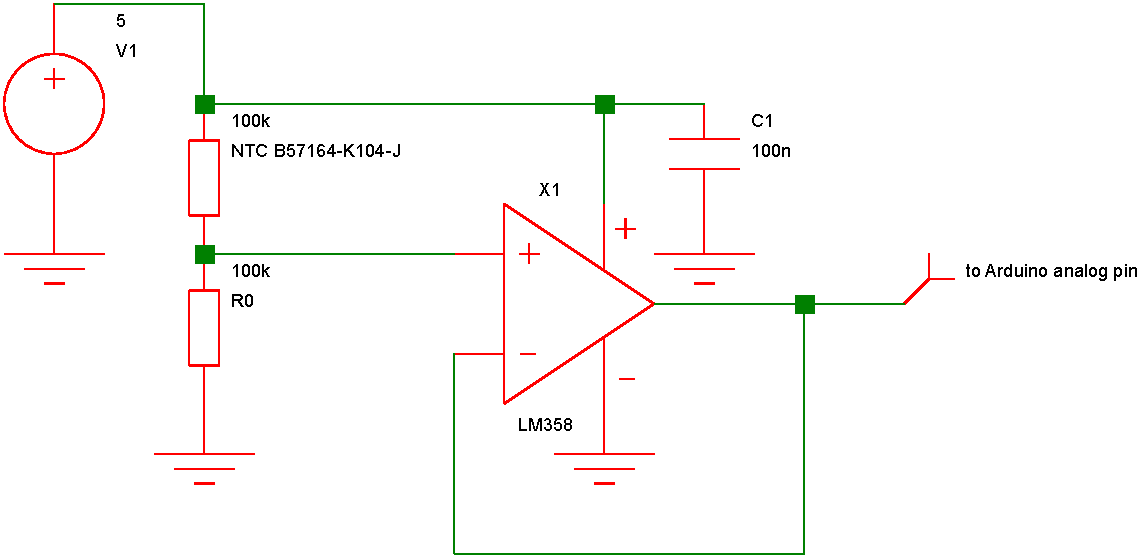
\includegraphics[width=14cm]{ntc_opamp_schematic}
\caption{Circuit for reading the NTC resistance with Op-amp.}\label{fig:tempcircuit}
\end{center}
\end{figure}

Figure \ref{fig:tempcircuit} shows the simplest possible circuit you can use for this purpose. The high input impedance of the op-amp ensures that there is basically no load on the voltage divider and we can use the simple formula which is only valid without load. There is then also virtually no current flowing through the NTC resistor which would heat it up.


\begin{figure}[H]
\begin{center}
  \centering
  \begin{minipage}[b]{0.4\textwidth}
    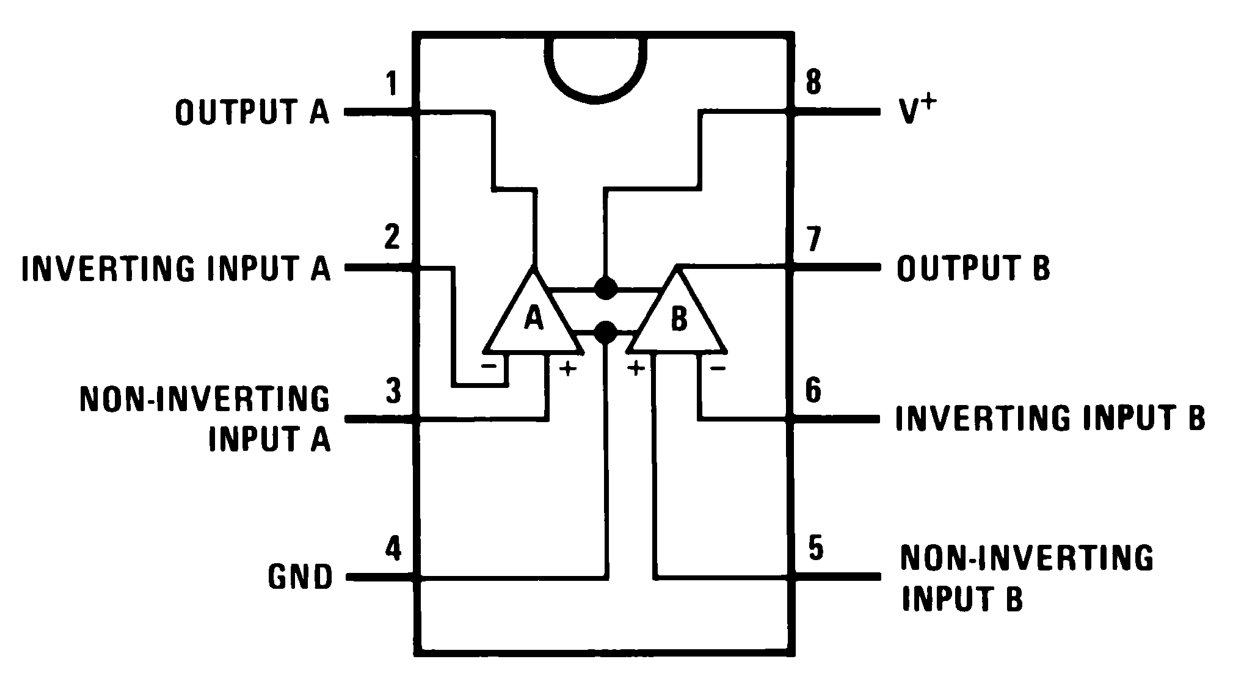
\includegraphics[width=\textwidth]{lm358pins}
  \end{minipage}
  \hfill
  \begin{minipage}[b]{0.5\textwidth}
    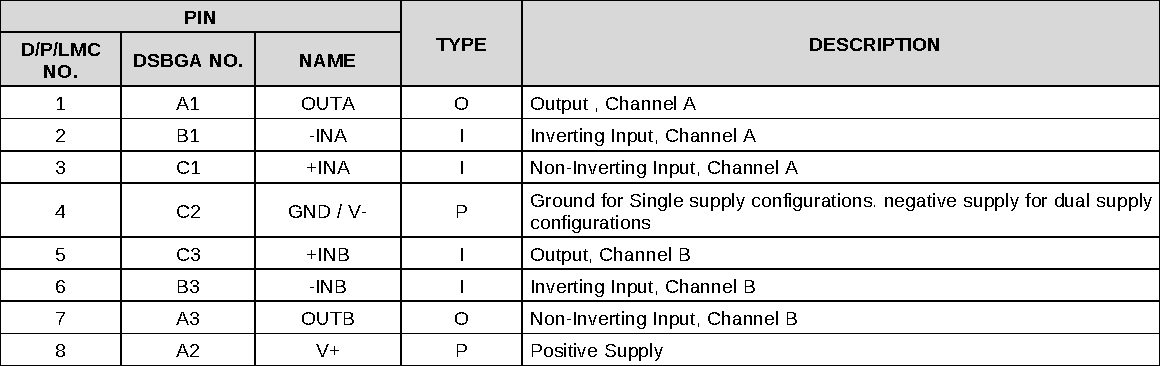
\includegraphics[width=\textwidth]{lm358table}
  \end{minipage}
\caption{Pin layout (left) and descriptions (right) of the LM358 Op-Amp. Source: datasheet from http://www.ti.com/lit/ds/symlink/lm158-n.pdf}\label{fig:tempcircuit2}
\end{center}
\end{figure}


\subsection{Calibration}\label{sec:calibration}

The NTC resistor we used for this experiment is not calibrated yet and therefore we obtain a relatively large error on the absolute temperature scale.
\vspace{0.5cm}
\begin{center}
\fbox{
  \parbox{0.9\textwidth}{
    \textbf{Task: calculate the uncertainty on the temperature we obtain from the following sources:}
    \begin{itemize}
    		\item B-constant of the NTC
    		\item resistance of the 100 k resistor (use 1\% resistors if possible)
    		\item resolution of the ADC
    		\item any other non-negligible uncertainty you find
    \end{itemize}
  }
}
\end{center}

By calibrating our device with an already calibrated reference device, we can reduce the systematic uncertainties. For this calibration we can use the Sensirion SHT21 temperature sensor or any equivalent device.

\vspace{0.5cm}
\begin{center}
\fbox{
  \parbox{0.9\textwidth}{
    \textbf{Task: calibrate your device by adjusting the B constant, such that its measured temperature matches the one measured with the reference device. Use the given uncertainty on the temperature of the reference device to calculate a new uncertainty for your B constant. How much does it improve?}
}
}
\end{center}


%END

\subsection{Heating}\label{sec:heat}
Since it is boring to measure a constant temperature, we build a simple heat load of 0.2-0.25 W with a couple of resistors.
\begin{itemize}
	\item calculate the resistors needed to have the correct power dissipation.
	\item bring the heating resistor and the temperature sensor close together to have as good thermal contact as possible.
\end{itemize}

Important: the temperature difference between the room temperature and the equilibrium temperature without cooling should be at least 5 degrees, better more (e.g. 10). 
If improving the thermal contact is not enough to heat up the NTC to more than 5 degrees above the room temperature, use the external power supply to provide power for the heating resistor.

\vspace{0.2cm}
\begin{center}
\fbox{
  \parbox{0.9\textwidth}{
    \textbf{Task: create a plot of the temperature vs. time (starting from room temperature) and determine the time constant of the temperature rise and estimate the equilibrium temperature from a fit.}
  }
}
\end{center}
\vspace{0.2cm}

\subsection{Cooling}\label{sec:cool}
Many electrical components will produce heat under load and may break at critical temperatures. That is why many of complex systems like computers require cooling. You will now build a system that controls a fan and can regulate it's rotation speed.
\begin{itemize}
	\item connect the fan to the breadboard, for the 4 pin header, the following conventions are used:
	\begin{itemize}
	    \item black: ground
	    \item yellow: 5V
	    \item green: tacho read-out (will be used later)
	    \item blue: PWM control
	\end{itemize}
	\item keep in mind that only a few of the digital pins (marked by "{\raise.17ex\hbox{$\scriptstyle\sim$}}" on the board) are able to use PWM, e.g. use digital pin 11
\end{itemize}

\subsection{Two-point controller}\label{sec:cool2}
Now we can finally build the full two-point controller.
\begin{itemize}
    \item define a low and high threshold, e.g. use the potentiometer for the high threshold and set the lower threshold a few degrees lower than the high one. both thresholds have to be in reach
	\item set the duty cycle of the fan to 100\% when above the high threshold
	\item set the duty cycle of the fan to 0\% when below the low threshold
	\item setting the PWM duty-cycle can be done using the \code{analogWrite()} function
\end{itemize}
Experiment with different set-points. What is the advantage of having two setpoints instead of a single threshold above we turn cooling on? What are the draw-backs of the two-point controller?

\vspace{0.5cm}
\begin{center}
\fbox{
  \parbox{0.9\textwidth}{
    \textbf{Task: create a plot of temperature vs. time with the two-point controller active which shows multiple periods.}
  }
}
\end{center}

\subsection{Read Out the Fan Speed}
We now wan to use the built-in Hall Effect Sensor (HES) of the fan to measure its rotation speed. In every rotation this sensor will produce two pulses we can count and then convert to revolutions per minute (\textbf{RPM}). The maximum (for 100\% duty cycle) according to the datasheet is 1900 RPM, with a tolerance of 10\%, the minimum is around 230 RPM.

\begin{itemize}
	\item calculate a rough estimate for the minimum frequency needed for reading the voltage on the tacho pin and be able to count the pulses? (Use Nyquist theorem) In practice, a much higher frequency should be used than the limit calculated above
	\item check the Arduino reference of \code{analogRead()} for the maximum frequency. Since we also have to do other work in the \code{loop()} function, the frequency should be also much less than the maximum. Make a reasonable choice.
    \item what is the expected uncertainty on the minimum and maximum RPM if we count pulses for 1 second?
	\item connect the tacho (green wire) of the fan to an analog pin of the Arduino, using a 10k pull-up resistor to 5V. (optional: figure out how to use internal pull-up resistor of the Arduino instead of a discrete component)
	\item what is the role of the pull-up resistor?
	\item count the pulses of the HES and convert the result to RPM. Is it within the range expected by the datasheet numbers?
	\item write the \ac{RPM} value to the serial output
\end{itemize}

\vspace{0.1cm}
\begin{center}
\fbox{
  \parbox{0.9\textwidth}{
    \textbf{Task: plot the fan RPM vs. the duty cycle. Which is the minimum duty cycle above which the fan starts to spin, and at which RPM? What is the maximum RPM for full duty-cycle?}
  }
}
\end{center}
\vspace{0.5cm}

Scanning the points for the different duty cycles should be done without flashing the device in between. Instead, the measurement programme (e.g. number of steps, seconds per step etc.) should be programmed into the Arduino or, alternatively, controlled by a Python program running on the computer which changes the parameters via the serial interface (see "Bi-directional communication with the computer" section below).

\subsection{Equilibrium temperature}
\begin{center}
\fbox{
  \parbox{0.9\textwidth}{
    \textbf{Task: plot the equilibrium temperature vs. the fan RPM. Make sure you measure long enough for each data point and give a reasonable estimate for the uncertainty that you obtain on the equilibrium value.}
  }
}
\end{center}
\vspace{0.5cm}

It might need few minutes to reach a stable equilibrium per point.


\subsection{PID Controller}
We have seen that with the two-point controller above, we could not exactly stabilize to a constant temperature and were suffering from under- and overshoot. Using a \ac{PID} controller can overcome both issues.
\begin{itemize}
	\item implement a \ac{PID} controller
	\item regulate cooling by the PWM duty-cycle of your fan
	\item tune your three parameters to have reasonably stable operation. (Perfect tuning is very complicated and does not have to done here.)
	\item create some plots with temperature vs. time, starting from different initial temperatures, which show converging temperature.
\end{itemize}

The output of the PID controller consists of three different terms, each having a tuneable coefficient.
\begin{itemize}
	\item proportional: proportional to the error, which is \code{error = temperature - setpoint}
	\item integral: proportional to the sum of all errors of previous steps
	\item derivative: proportional to the difference in error compared to last step
\end{itemize}

In practice, there are few more things to consider
\begin{itemize}
    \item using a timer, perform the PID calculations between every 100 ms and every second. You should not use longer values to be fast enough in response and not too much shorter values to be not susceptible to noise.
    \item use a discrete digital low-pass filter on your measured temperature if it is noisy.
    \item convert your PID response to a duty\_cycle between 0 and 255 to be used in \code{\meth{analogWrite}(\var{PIN\_FAN\_PWM}, duty\_cycle)}. 
\end{itemize}

\begin{center}
\fbox{
  \parbox{0.9\textwidth}{
    \textbf{Task: Optimize the three parameters reasonably well to have fast convergence and low fluctuations after a certain time and plot the temperature vs. time. Also de-tune your parameters to produce slow convergence and/or overshooting/oscillations and show both curves in one plot.}
  }
}
\end{center}

\vspace{0.5cm}

A low-pass filter can be used to filter out high frequency fluctuations (noise) on the measured temperature. It can be implemented in it's simplest form with

\noindent\begin{minipage}{\textwidth}
\begin{lstlisting}[language=Arduino]
temperature = (1-LOWPASS_ALPHA) * temperature + LOWPASS_ALPHA * temperature_current;
\end{lstlisting}
\end{minipage}

where \code{temperature\_current} is the actual reading from the sensor and \code{temperature} (which has to be properly initialized once to be the sensor reading!) the output of the filter. \code{\var{LOWPASS\_ALPHA}} and the interval between two measurements $\Delta t$ control the cut-off frequency of the lowpass filter. Set it to a reasonable value which suppresses the noise and is still fast enough for the timescale of temperature changes we expect (order of few degrees per second). It can also be computed analytically:

\begin{equation}
\alpha = \frac{\Delta t}{\tau + \Delta t}
\end{equation}

where $\tau$ is the characteristic time constant of the low-pass filter (corresponds to RC time of a RC filter). Setting $\alpha = 0$ makes it infinitely fast, so the output is equal to the input, where as $\alpha = 1$ makes the response infinitely slow, so the output would stay constant at its initial value.

\subsection{Advanced tasks}

\fbox{
  \parbox{0.9\textwidth}{
    \textbf{All of the following tasks are optional. They can be used to replace some of the other tasks if agreed on with the assistant.}
  }
}


\subsection{Fit heating/cooling(Advanced)}
Take the two-point controller and set the two setpoints far from each other, but still in achievable range. For heating and cooling process, find a suitable function to describe the data and perform a fit of the model to data. List the fit parameters (with uncertainties!) and repeat this for several cycles. Take special care on correlation of input uncertainties in the fit and explain in the report why this is an issue here and what effect it would have to neglect correlations. Also look at the uncertainties and correlations of the fitted parameters.
Are the uncertainties obtained by repeating the experiment consistent with the uncertainties from the fit? If not discuss why.

\subsection{Bi-directional communication with the computer (Advanced)}
Until now we only read values from the device, but we can also write commands from the computer to the Arduino using the serial interface.
\begin{itemize}
	\item instead of using the potentiometer to set the threshold, implement a way to set the threshold via serial commands
	\item one can use the SCPI protocol as a reference, e.g. set the threshold to 32 degrees with the command "SET:THR 32"
	\item which other commands are necessary to run the measurements from above section without hardcoding the measurement programme (e.g. number of steps, seconds per step etc.)?
	\item write a Python script to perform the measurements from above section via sending SCPI style commands to the Arduino
\end{itemize}


\subsection{Use of other components (Advanced)}
There is also a bunch of other components available which can be used to extend your Arduino project. Among them:
\begin{itemize}
	\item ultra-sonic distance sensor
	\item electric current sensor
	\item infrared leds and sensor
	\item electro magnet
	\item Piezzo vibration sensor
	\item 96x96 pixels OLED display
	\item Servo motor
	\item ...
\end{itemize}

Ask the assistants for more information if you are interested in using them. For example you could use the distance sensor and servo motor to keep an object at a fixed position relative to another moving one.


\subsection{I2C protocoll debugging (Advanced)}
Many of the Grove components communicate via I2C bus protocol. Using a digital oscilloscope, it is possible to look at the I2C signal and manually decode it on the scope. Use the Grove RBG LCD display, initialize it and periodically write text to the display and set the color. Spy on the commuication, find out the the device IDs of the 2 devices connected to the bus. What do they correspond to? Compare with the library of the Grove display. Record a short communication of a few bytes and decode it.















